\subsection{App}

\subsubsection{Konfigurationsdatei-config.xml}

Um die Metadaten der App zu konfigurieren, um bestimmte Einstellungen zu treffen oder um Plugins zu laden wird die Datei config.xml benötigt. Diese Konfigurationsdatei wird zusammen mit allen anderen Dateien in das ZIP-Paket gespeichert und für den PhoneGap build hochgeladen.\\
Die config.xml besteht grundsätzlich aus XML-Code.\\
Am Anfang der Datei steht ein Widget-Tag in welchem die ID der Applikation und die Versionsnummer angegeben werden.\\
 
\lstinputlisting[style=custom, language=xml, caption={config.xml}, label={lst:widget}, firstline=2, lastline=6]{sources/app/config.xml}


Weitere Tags sind\\
\begin{tabular}{llpipe}
   <name></name>&Damit wird der Name der App angegeben\\
   <description></description>&Darin wird eine Beschreibung der App\\
    						&geschrieben\\
   <author email="help@sis.htlinn.ac.at"></author>&Zwischen diesen Tags wird angegeben\\
    											&wer die App erstellt hat.\\
   <icon src="images/icon.png" />&Mit diesem Tag kann man den Pfad des\\
   								&App-Icons angeben.\\
   <gap:splash src="images/splash.png" />&Mit diesem Tag kann man den Pfad des\\
    									&Splashscreens angeben.\\
   <access origin="http://sis.htlinn.ac.at"/>&Mit dem Access-Tag gibt man an auf\\
   											&welche Webseiten die App zugreifen,\\
   											&bzw. welche Webseiten die App laden darf.\\
   <manifest> </manifest>&Das Manifest Tag wurde verwendet um\\
   						&das Android-Manifest zu erstellen,\\
   						&darin kann man	Berechtigungen für die\\
   						&Android-App einstellen. Das Manifest\\
   						&wäre in diesem Fall aber nicht notwendig\\
   						&gewesen.\\
   <gap:plugin name=" " version="" />&Mit diesem Tag werden Plugins eingebunden.\\
   \\
 \end{tabular}

Für iOS wird das Icon in vielen verschiedenen Größen benötigt, damit die App für alle Geräte angepasst ist. Darum wurden zusätzlich noch zwölf Icons erstellt und in der config.xml eingebunden. Damit die Icons auch richtig zugewiesen werden, werden dem Icon-Tag noch jeweils ein Attribut für die Höhe und die Breite des Bildes und ein Attribut um das richtige Betriebssystem anzugeben, mitgegeben.\\
Beispiel:\\

\lstinputlisting[style=custom, language=xml, caption={config.xml}, label={lst:widget}, firstline=32, lastline=32]{sources/app/config.xml}
	

Bei den Splashscreens (das Bild das beim Starten der App erscheint) müssen auch mehrere Formate eingebunden werden.
Um zu vermeiden, dass es durch PhoneGap zu Problemen mit der Kommunikation zwischen der App und dem Server kommt wurde die URL des Servers (https://sis.htlinn.ac.at), mit Hilfe des Access-Tags als Ausnahme hinzugefügt.\\

Bei den Preferences wurde eingestellt, dass die Applikation keine Berechtigungen hat,\\

\lstinputlisting[style=custom, language=xml, caption={config.xml}, label={lst:widget}, firstline=84, lastline=84]{sources/app/config.xml}

Dadurch wird beim Installieren der App, die Verbindung mit dem Internet als einzige angeforderte Berechtigung angezeigt. Diese Berechtigung kann bei PhoneGap-Apps nämlich nicht abgestellt werden.\\

Weiters wurde mit den Preferences noch eingestellt, dass die App im Fullscreen-Modus betrieben wird und das die App bevorzugt auf dem externen Speicher installiert wird.\\


\subsubsection{Erstellen einer App mit PhoneGap}
Um unsere App zu erstellen wurde die Onlinevariante von PhoneGap, PhoneGap Build, verwendet. Dazu muss man sich zuerst bei AdobeSystems registrien, das kann man aber kostenlos machen.\\
Danach meldet man sich unter https://build.phonegap.com an und kommt es erscheint folgende Seite.\\

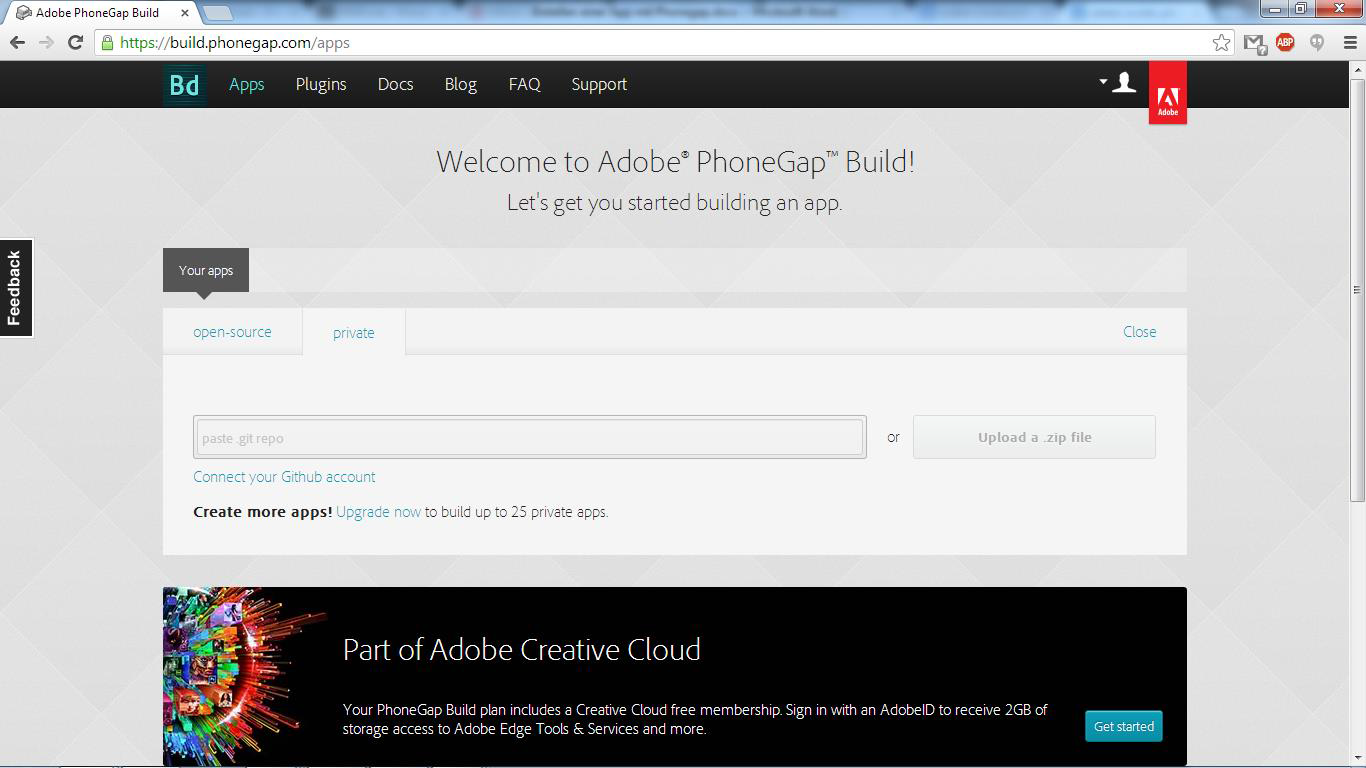
\includegraphics[keepaspectratio=true, width=14cm]{images/phoneGap/PhoneGap1.png}

Hier muss man nun den Reiter „private“ auswählen, damit man die Appdaten in Form eines Zipfiles hochladen kann.
Um Fortzufahren muss man nun das Zipfile, in welchem die Daten für die App(alle HTML, CSS und JavaScript-Files) gespeichert sind hochladen.\\
Ist das geschehen versucht die Webseite die Apps für Android, WindowsPhone und iOS zu compilieren. Für Android und WindowsPhone funktioniert das auch, falls der Code und vor allem die Konfigurationsdatei korrekt sind, aber bei iOS kommt eine Fehlermeldung. Denn um Apps für iOS zu erstellen benötigt man Zertifikate, welche man nur als Apple-Developer bekommt.\\
Nach dem ersten Build sieht man, dass für den Appnamen das Appsymbol und weitere Einstellungen die Einstellungen aus der config.xml übernommen wurden.\\

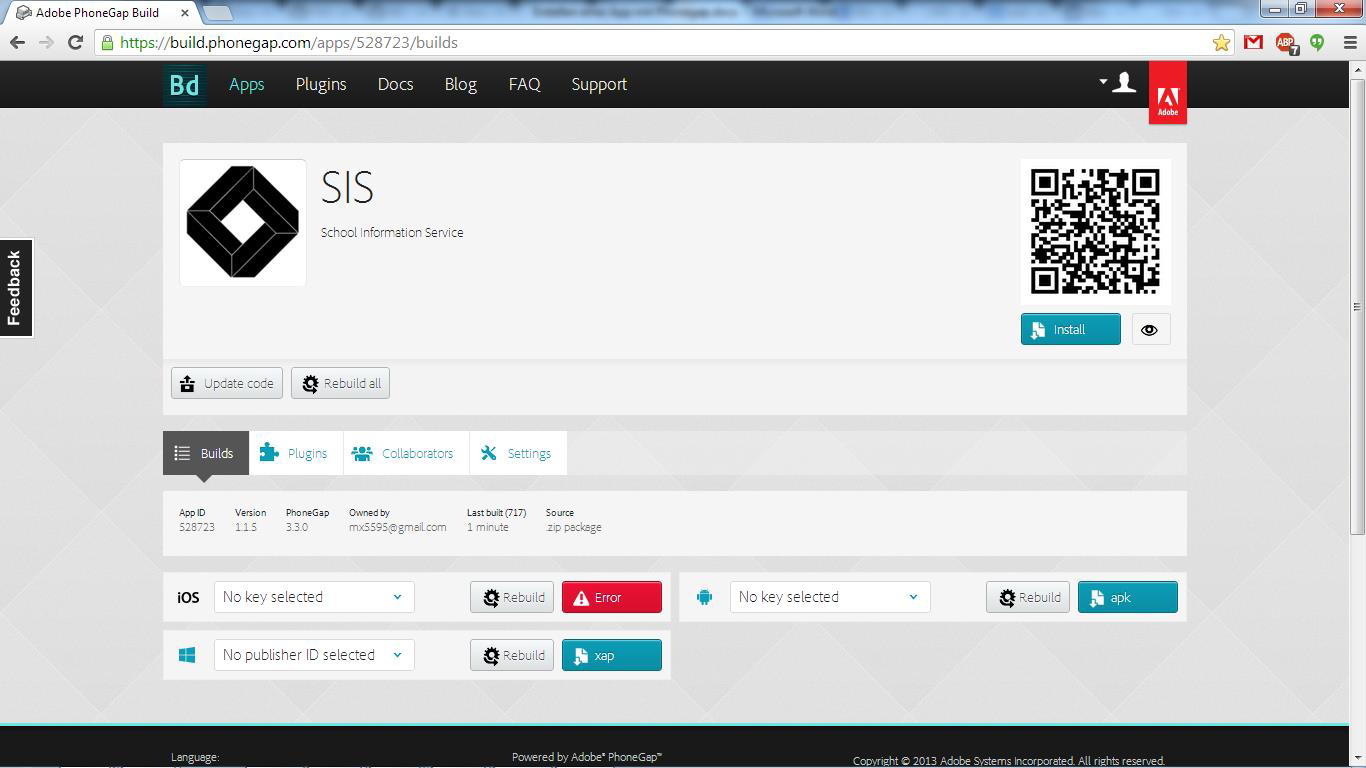
\includegraphics[keepaspectratio=true, width=14cm]{images/phoneGap/PhoneGap2.png}

Um die Applikation zu updaten müssen alle Dateien die verändert wurden in der ZIP-Datei ausgetauscht werden und die ZIP-Datei muss neu hochgeladen werden. Dazu klickt man einfach auf „Update code“ und wählt dann die gewünschte ZIP-Datei aus.\\
Die Android-App und die App für WindowsPhone kann man jetzt bereits testen. Bei Android muss man dazu nur zuerst in den Einstellungen, im Untermenü Anwendungen, die Option Unbekannte Quellen aktivieren. Dann kann man einfach das APK-File auf das Gerät laden(entweder direkt mit dem Gerät downloaden oder via USB, Bluetooth, etc. auf das Gerät laden) und ausführen, und die Applikation wird wie jede andere App installiert. Nun kann man die App nutzen.\\
Die App auf dem WindowsPhone zu nutzen ist etwas umständlicher. Entweder man stellt die App direkt in den Store oder wenn man sie nur testen möchte, kann man die App auch mit Hilfe von Developer Tools direkt auf das Smartphone laden und Testen.\\
Damit die Android-App in den Play-Store von Google geladen werden kann, muss diese zuerst noch signiert werden. Dazu muss eine Keystore-Datei erzeugt werden mit welcher die App signiert werden kann.\\
Dieses Keystore-File kann man selbst erstellen, sofern man die JDK (Java Development Kit) installiert hat. Um den Schlüssel zu erstellen muss man die Eingabeaufforderung öffnen und in das Verzeichnis der JDK wechseln, als nächstes kann man mit dem Befehl keytool und einigen Parametern ein Keystotre-File erstellen.\\
Beispielbefehl:\\

\begin{lstlisting}
$ keytool -genkey -v -keystore my-release-key.keystore -alias alias_name -keyalg RSA -keysize 2048 -validity 10000
\end{lstlisting}

Nachdem dieser Befehl eingegeben wurde wird man noch aufgefordert, den Namen des Entwicklers oder Entwicklerteams, die Nationalität und einige weiter Angaben einzugeben. Zuletzt muss noch ein Passwort angegeben werden, dieses wird benötigt um den Schlüssel zu entsperren wenn er bei PhoneGap genutzt wird.\\
Nun wird eine Datei, in diesem Fall mit dem Namen my-release-key.keystore, erstellt.\\
Wenn man nun das Dropdownmenü neben dem Androidsymbol öffnet,\\

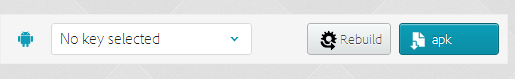
\includegraphics[keepaspectratio=true, width=7cm]{images/phoneGap/PhoneGap3.png}

erscheint ein Punkt „add a key…“. Wenn man diesen Punkt auswählt wird man aufgefordert eine Datei hochzuladen, dabei handelt es sich um die Keystore-Datei welche zuvor erzeugt wurde. Dann muss man dem Schlüssel noch einen Namen geben und bestätigen.\\
Nun kann man in diesem Dropdownmenü den hochgeladenen Schlüssel auswählen, um ihn zu nutzen muss man zuerst noch ein Passwort eingeben, das ist jenes Passwort welches zuvor beim erstellen des Keystore-Files angegeben wurde. Wenn man nun einen Rebuild macht bekommt man eine Android-Release-App welche auch im Play-Store veröffentlicht werden kann.
Bei iOS benötigt es bereits ein Entwicklerzertifikat um eine Debug-App zu erstellen. Um ein solches Zertifikat zu erstellen muss man bei Apple als Developer angemeldet sein und 99\$ im Jahr bezahlen.\\
Für dieses Projekt wurde der Apple-Enterprise-Account der Schule genutzt. Man benötigt nur eine Apple ID (Registrierung unter https://developer.apple.com/register/ ), mit dieser kann man dann von einem Administrator (in unserem Fall Direktor Laner) zum Account hinzugefügt werden.\\
Nachdem man zum Enterprise-Programm hinzugefügt wurde, muss man das MemberCenter (https://developer.apple.com/membercenter/ ) öffnen.\\

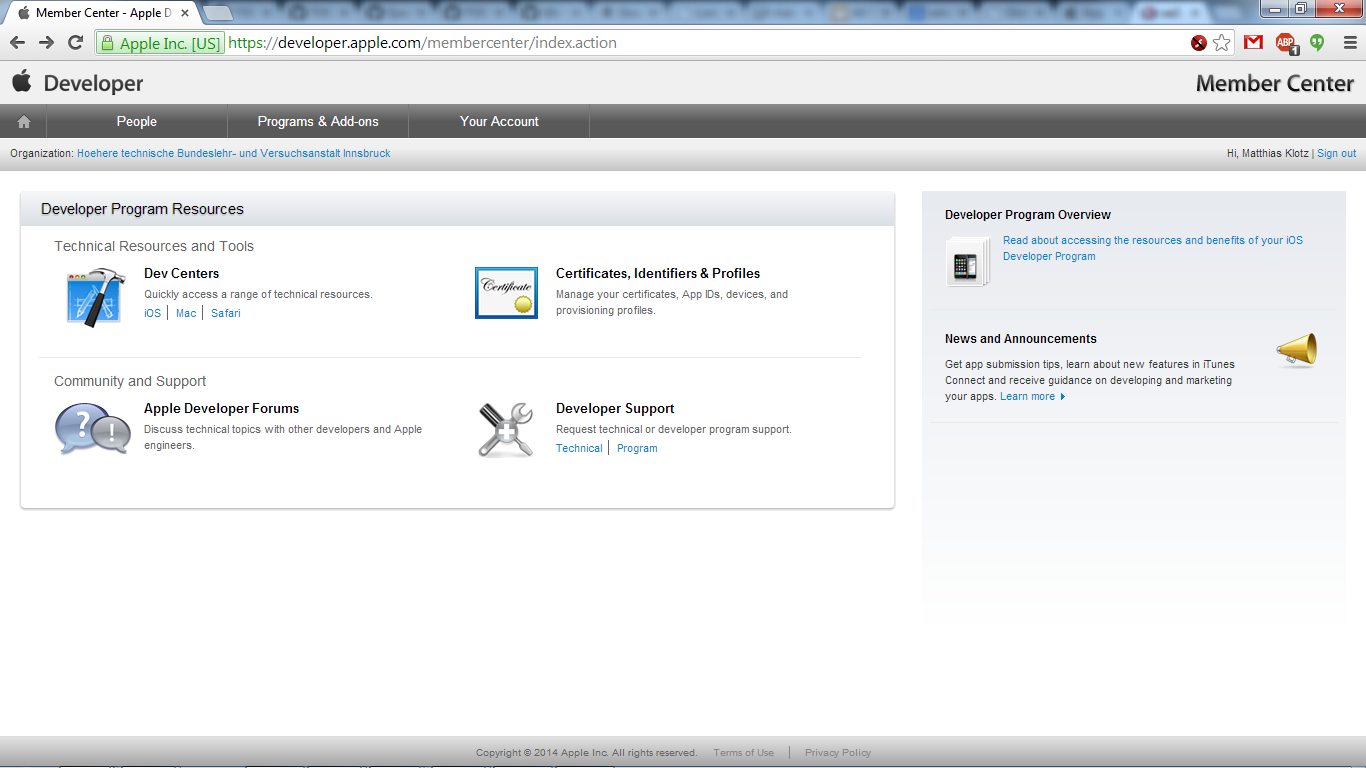
\includegraphics[keepaspectratio=true, width=14cm]{images/phoneGap/AppleMemberCenter1.png}

Unter „Certificates, Indentifiers \& Profiles“ kann man nun die benötigten Zertifikate erstellen und downloaden.\\

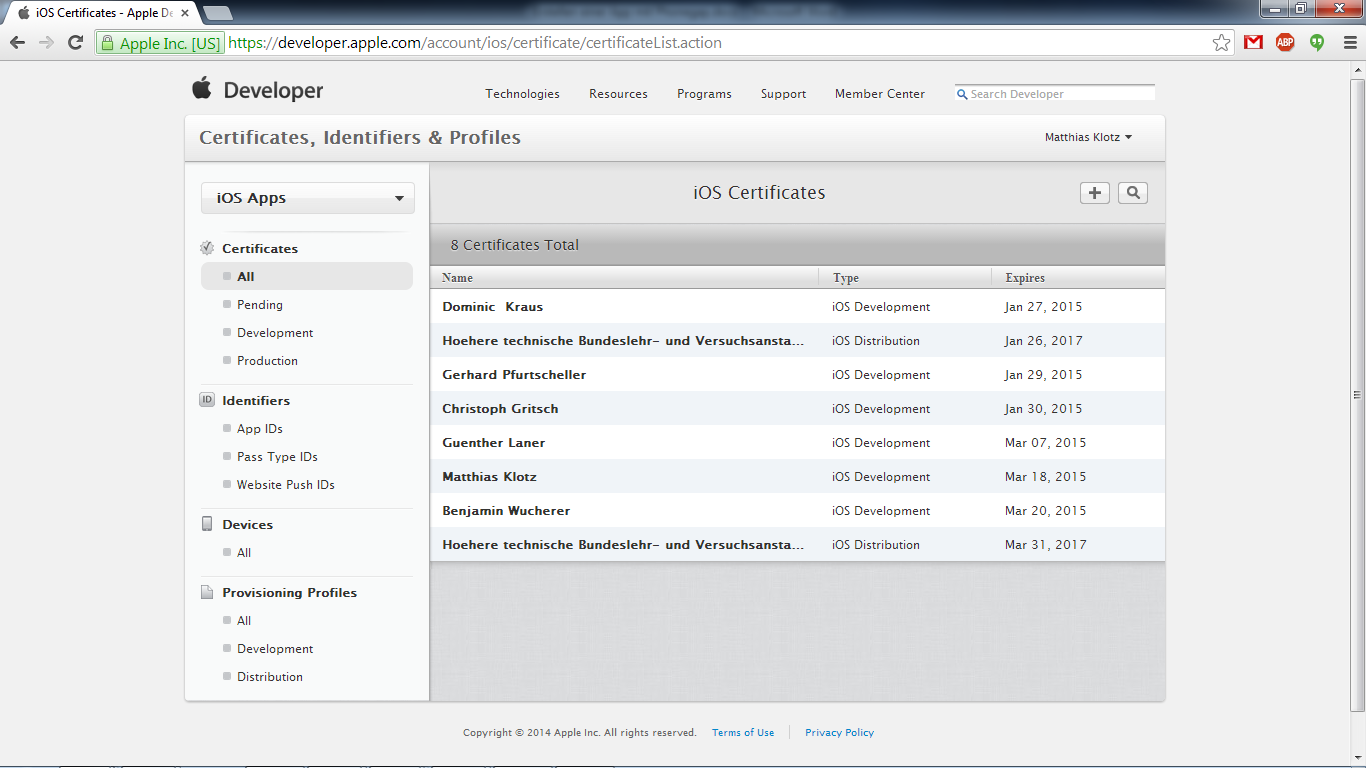
\includegraphics[keepaspectratio=true, width=14cm]{images/phoneGap/AppleMemberCenter2.png}

Um ein neues Zertifikat zu erstellen öffnet man zuerst den Menüpunkt Certificates und klickt dann auf das Plus-Symbol in der rechten oberen Ecke des Fensters. Daraufhin erscheint der Assistent zum erstellen eines neuen Zertifikates.
Als erstes wird gefragt wozu das Zertifikat verwendet wird. Dabei muss man zuerst unterscheiden ob es sich um ein Development oder ein Production Zertifikat handelt. Bei einem Development Zertifikat
werden bestimmte Developergeräte angegeben auf welchen die Applikation getestet werden kann ohne dass sich die App im Appstore befindet.\\
Ein Production Zertifikat wird hingegen benötigt um eine App zu erstellen welche für alle Geräte nutzbar ist, diese App muss dann aber für gewöhnlich über den Appstore veröffentlicht werden.\\
Für dieses Projekt wurden beide Varianten erstellt und genutzt.\\
Bei beiden Varianten wird man im nächsten Schritt aufgefordert einen CSR (Certificate Signing Request) hochzuladen. Diese Datei erhält man indem man die Schlüsselbundverwaltung bei Mac OS X öffnet und im Menü Datei unter Zertifikats Assistent, „neues Zertifikat erstellen“ wählt. Dabei wird man aufgefordert eine E-Mail-Adresse und den eigenen Namen anzugeben, wichtig ist das der Punkt als Datei speichern ausgewählt wird.\\
Nach Angabe der Informationen kann man nun eine CSR-Datei abspeichern. Diese Datei wird als nächstes bei der Erstellung des Zertifikates auf der Apple-Website hochgeladen. Nun kann man das Zertifikat erstellen und downloaden.
Als nächstes muss noch ein Provisoining-File erstellt werden. Dazu wechselt man einfach auf den Menüpunkt Provisioning Profiles und klickt dann auf das selbe Symbol wie zuvor bei den Zertifikaten. Es erscheint wieder ein Assistent der bei der Erstellung des Provisioning Profils hilft. Als erstes muss man wieder Angeben wozu das Provisioning Profile benötigt wird. Wenn man zuvor ein Development Zertifikat erstellt hat muss man nun wieder Development auswählen, hat man aber zuvor ein Production Zertifikat erstellt muss man nun Distribution auswählen. Im nächsten Schritt muss noch eine App-ID gewählt werden, dazu wurde einfach eine bereits existierende ID ausgewählt. Als nächstes wird nach einem Zertifikat gefragt, hier wird dass zuvor erstellte Zertifikat ausgewählt.\\
Falls ein Development Provisioning Profile erstellt wird, wird man noch nach den Entwicklergeräten gefragt, hier muss man sein eigenes iPhone, welches zuvor unter Devices hinzugefügt wurde, auswählen.\\
Wenn man soweit ist kann man auch das Provisioning Profile generieren und herunterladen.\\
Da für PhoneGap aber ein privater Schlüssel in Form eines P12-Files benötigt wird, muss dieser erst aus dem Zertifikat exportiert werden. Dazu muss man zuerst das heruntergeladene Zertifikat in die Schlüsselbundverwaltung importieren, dann wählt man das soeben importierte Zertifikat aus, nun klickt man mit der rechten Maustaste darauf und wählt exportieren aus und exportiert das Zertifikat als P12-Datei.\\
\\
Wenn man nun das Dropdownmenü neben dem Applelogo öffnet,

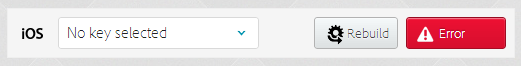
\includegraphics[keepaspectratio=true, width=7cm]{images/phoneGap/PhoneGap4.png}

erscheint ein Punkt „add a key…“. Wenn man diesen Punkt auswählt wird man aufgefordert zwei Dateien hochzuladen, eine P12-Datei und ein Provisioning-File, dabei handelt es sich um die beiden Dateien die gerad erstellt wurden. Wenn diese Dateien hochgeladen wurden kann die Applikation erstellt werden.\\
Hat man ein Developer-Zertifikat erstellt kann die erstellte App nur auf den in dem Zertifikat bestimmten Geräten betrieben werden, wurde aber ein Distribution Zertifikat erstellt kann die App nun auf allen iOS-Geräten verwendet werden.\\
Um die App für den App-Store zu builden wurden uns die Zertifikate von Direktor Günther Laner zur Verfügung gestellt, da die Applikation über den Developer Account des Direktors veröffentlicht wird.\\

% Söö: Wie wurde die App erstellt?
% Ich weiß das leider nicht so genau, deswegen kann ich dir nicht vorschlagen, was du erwähnen sollst, und was nicht. 
% Die Generierung des Stunden- und Supplierplans musst du nicht mehr erwähnen.
% 
% Hier dürfen auch auch Sourcecode-Teile vorkommen.
% Wenn Sourcecodes: jeweilge File in den Ordner /sources/ in einen Unterordner packen und mit folgendem Befehl includieren:
%
%
% \lstinputlisting[style=custom, language=php, caption={Dateiname}, label={lst:content_imple_timetables_labelname}]{sources/ordner/datei.php}
%
% Als weitere Eigenschaft kannst du die Zeilen angeben: [firstline=300, lastline=500]
% Damit nicht alles reinkopiert wird.